\documentclass[a4paper, 12pt]{article}

\def \patha {} %Pfad zu den Dateien Preamble.tex, Commands.tex, Erwartungsbild.tex

\input{\patha/Preamble.tex}

\onehalfspacing

\newcommand{\KopfzeileBlank}{true}
\newcommand{\FACH}{Informatik}
\newcommand{\KLASSE}{Kl. 5}
\newcommand{\DATUM}{XX.YY.ZZZZ}
%% Über den jeweiligen Typ wird bei Klassenarbeit und Leistungskontrolle das Erwartungsbild und der Notenspiegel als anhängende Seite kompiliert. Der Befehl \aufgabe besitzt beim Typ Arbeitsblatt einen Parameter für die Aufgabenstellung. Bei den Typen Klassenarbeit und Leistungskontrolle kommen noch zwei weitere Parameter für die Punktzahl und das Erwartungsbild hinzu.
\newcommand{\TYP}{Arbeitsblatt}
%\newcommand{\TYP}{Klassenarbeit}
%\newcommand{\TYP}{Leistungskontrolle}
\newcommand{\EINHEIT}{Scratch}
\newcommand{\THEMA}{Eine Geschichte gestalten}
\newcommand{\LEHRER}{N.N.}
\newcommand{\TIME}{Zeit}
\newcommand{\NTA}{Hier ist Platz für Nachteilsausgleiche!}
%% Dieser "Switch" bewirkt, dass für Lückentexte die Lösung angezeigt oder ausgeblendet wird. Aktuell werden die Lücken jedoch noch nicht berücksichtigt. Vielleicht gibt es auch eine bessere Lösung für diesen "Switch"...
%\newcommand{\LOSUNG}{true}
\newcommand{\LOSUNG}{false}

%\input
\input{\patha/Commands.tex}

\begin{document}

\large
\TITEL

\subsection*{Die Geschichte}
Der Hund Bello sieht eine Banane und wundert sich, was das ist. Danach läuft er zu der Banane und stellt fest, dass er keine Bananen mag.

\subsection*{Das Programm}
Gestalte die Geschichte von Bello in Scratch. Das Programm soll folgende Figuren besitzen:
\begin{enumerate}
	\item Den Hund Bello (Figur Dog2) an der Position x: -180; y: -82
	\item Die Bananen (Figur Bananas) an der Position x: 190; y: -82
\end{enumerate}
\vspace{1em}
Wähle für die Geschichte eine passende Bühne.
\vspace{1em}

Das Programm soll nach folgendem Ablauf funktionieren:

\begin{enumerate}
	\item Das Programm wird mit einem Klick auf die Fahne gestartet.
	\item Bello wechselt zu Kostüm \glqq{}dog2-c\grqq{}.
	\item Bello geht zur Position \glqq{}x: -180 y: -82\grqq{}.
	\item Bello denkt für \textbf{2} Sekunden \glqq{}Nanu, was ist das denn?\grqq{}.
	\item Bello läuft solange, bis er die Banane erreicht. Hierzu soll folgende Schrittfolge wiederholt werden:\newline 1. Wechsle zum nächsten Kostüm\newline 2. Gehe 40er Schritt\newline 3. Warte 0.3 Sekunden
	\item Sobald Bello die Banane erreicht hat wechselt er wieder zu Kostüm \glqq{}dog2-c\grqq{}.
	\item Bello denkt für \textbf{2} Sekunden \glqq{}Hmm... Doch nichts für mich.\grqq{}.
\end{enumerate}

\subsection*{Verwendbare Blöcke}
Verwende für das Programm folgende Blöcke:

\begin{minipage}{0.33\textwidth}
	
\includegraphics{blau_1.png}
\end{minipage}
\begin{minipage}{0.33\textwidth}
	
\includegraphics{blau_2.png}
\end{minipage}
\begin{minipage}{0.33\textwidth}
	
\includegraphics{lila_1.png}
\end{minipage}

\begin{minipage}{0.49\textwidth}
	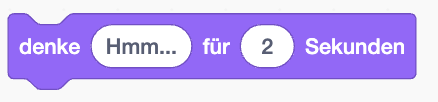
\includegraphics{lila_2.png}
\end{minipage}
\begin{minipage}{0.49\textwidth}
	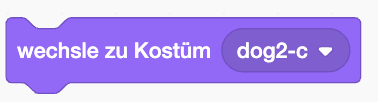
\includegraphics{lila_3.png}
\end{minipage}

\begin{minipage}{0.33\textwidth}
	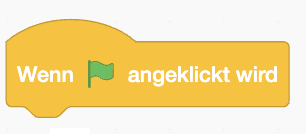
\includegraphics{orange_1.png}
\end{minipage}
\begin{minipage}{0.33\textwidth}
	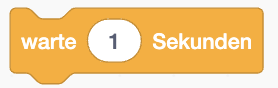
\includegraphics{orange_2.png}
\end{minipage}
\begin{minipage}{0.33\textwidth}
	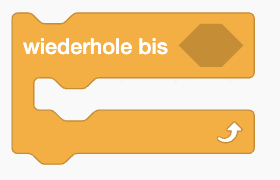
\includegraphics{orange_3.png}
\end{minipage}

\begin{minipage}{0.33\textwidth}
	
\includegraphics{tuerkis_1.png}
\end{minipage}


%\input
\label{LastPage}
\normalsize
\ifthenelse{\equal{\TYP}{Klassenarbeit}}{
\input{\patha/Erwartungsbild.tex}}
{}
\ifthenelse{\equal{\TYP}{Leistungskontrolle}}{
\input{\patha/Erwartungsbild.tex}}
{}


\end{document}